\noindent
\begin{tabular}{cc}
\begin{minipage}{0.95\textwidth}
\begin{exerciseS}[Motore a getto]
 Un aereo vola alla velocità $V=250 \, m/s$ alla quota $z=10000 \, m$, dove la pressione e la temperatura atmosferica sono $P_0 = 26500 \, Pa$ e $T_0 = 223.25 \, K$, spinto dal motore a getto rappresentato in figura. Sapendo che:
 \begin{itemize}
  \item $0 \rightarrow 1$: la presa d'aria è progettata per ottenere una compressione adiabatica ideale (isentropica), con $P_1/P_0 = 1.5$;
  \item $1 \rightarrow 2$: il compressore ideale ha una sezione di ingresso $A_1 = \dots$ e produce un rapporto di pressione totale $P_2^t/P_1^t = 40.0$, tramite una trasformazione adiabatica ideale;
  \item $2 \rightarrow 3$: il combustore garantisce una perfetta combustione mantenendo costante la pressione totale al suo interno $P_2^t = P_3^t$; il flusso di calore prodotto dalla combustione è uguale a $\dot{Q}_c = \dot{m}_f \Delta h_c$, dove $\dot{m}_f$ è il flusso di massa di combustibile e $\Delta h_c = 46 \, MJ/kg$ il suo potere calorifico; la temperatura totale all'ingresso della turbina è $T_4^t = 1600 \, K$;
  \item $3 \rightarrow 4$: nella turbina avviene un'espansione adiabatica ideale, in modo tale da garantire la potenza necessaria a mantenere in moto il compressore;
  \item $4 \rightarrow 5$: nell'ugello avviene un'espansione adiabatica ideale, che porta il gas a espandersi fino alla pressione ambiente $P_5 = P_0$.
 \end{itemize}
 Si considerino tutti i componenti meccanici ideali, si trascurino gli effetti viscosi dove possibile e si consideri l'aria e la miscela di gas combusti come un gas biatomico ideale, con costante dei gas $R = 287 \, J/(kg \, K)$ e calori specifici costanti.
 \newline \noindent
Viene chiesto di calcolare:
\begin{itemize}
 \item il rapporto in massa tra flusso di combustibile e flusso di aria, $f = \dot{m}_f / \dot{m}_a$;
 \item la spinta $T$ fornita dal motore.
\end{itemize}
\end{exerciseS}
\end{minipage}
\end{tabular}
\begin{figure}[h!]
 \centering
 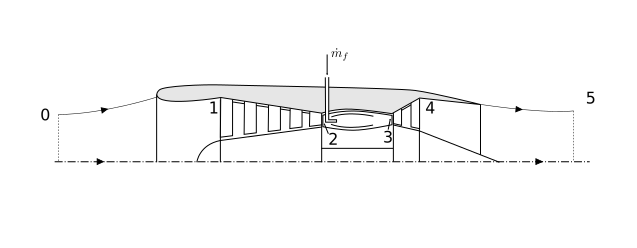
\includegraphics[width=0.95\textwidth]{./fig/jet_engine}
\end{figure}

\sol

\partone
Durante lo svolgimento dell'esercizio vengono utilizzati i bilanci integrali di massa,
\begin{equation}
 \dfrac{d}{dt} \displaystyle\int_{V(t)} \rho + \oint_{S(t)} \rho (\bm{u}-\bm{v}) \cdot \bm{\hat{n}} = 0 \ ,
\end{equation}
quantità di moto,
\begin{equation}
 \dfrac{d}{dt} \displaystyle\int_{V(t)} \rho \bm{u} + \oint_{S(t)} \rho \bm{u} (\bm{u}-\bm{v}) \cdot \bm{\hat{n}}= \int_{V(t)} \bm{f} + \oint_{S(t)} \bm{t_n} \ ,
\end{equation}
ed energia totale,
\begin{equation}
 \dfrac{d}{dt} \displaystyle\int_{V(t)} \rho e^t + \oint_{S(t)} \rho e^t (\bm{u}-\bm{v}) \cdot \bm{\hat{n}}= \int_{V(t)} \bm{f} \cdot \bm{u} + \oint_{S(t)} \bm{t_n} \cdot \bm{u} - \oint_{S(t)} \bm{q} \cdot \bm{\hat{n}} + \int_{V(t)} \rho r \ .
\end{equation}
In particolare, il bilancio di quantità di moto permette di ricavare la formula della spinta del motore in funzione del flusso di quantità di moto attraverso un volume di controllo opportunamente scelto. Il bilancio di energia totale permette di analizzare i singoli componenti del motore. 

\vspace{0.5cm}
\parttwo
Per risolvere il problema, è necessario ricavare la spinta del motore in funzione della portata massica trattata e della differenza di velocità del fluido in ingresso e in uscita dal motore. Successivamente viene analizzato il sistema motore per calcolare la velocità di efflusso dei gas. Si considera il problema stazionario, con forze di volume $\bm{f}$ trascurabili. Si svolge uno studio ``quasi-1D'' considerando variabili uniformi sulle varie sezioni del motore.
%
% \newline \noindent \textbf{Formula della spinta.}
\paragraph{Formula della spinta.}
Nell'ipotesi che la pressione dei gas in uscita dall'ugello sia uguale alla pressione ambiente, il bilancio di quantità di moto del fluido trattato dal motore permette di ottenere la stima della trazione generata dal motore,
\begin{equation}
 T = \dot{m}_5 V_5 - \dot{m}_0 V_0 = \dot{m}_0 ( V_5 - V_0 ) + \dot{m}_f V_5 \ .
\end{equation}
Per ricavare la trazione $T$ è necessario ricavare i valori del flusso di massa d'aria ingerito dal motore, il flusso di combustibile e la velocità di efflusso dei gas combusti, studiando in dettaglio il fluido all'interno del motore
% 
% \newline \noindent \textbf{Analisi del motore.}
\paragraph{Analisi del motore.}
Si studia l'evoluzione della corrente che attraversa il motore.
\begin{itemize}
 \item $0 \rightarrow 1$, presa d'aria: l'aria che approccia l'ingresso del compressore $S_1$ subisce una compressione libera adiabatica ideale. Dato lo stato termodinamico TD(0), con $\rho_0 = P_0/ (R T_0) = 0.414 \, kg/m^3$, e il rapporto di pressione $P_1 / P_0$, è possibile calcolare lo stato termodinamico TD(1):
 \begin{equation}
   P_1 = \left( \dfrac{P_1}{P_0} \right) P_0 = 39750 \, Pa \qquad , \qquad
\rho_1 = \left( \dfrac{P_1}{P_0} \right)^{\frac{1}{\gamma}} \rho_0 = 0.553 \, kg/m^3 \ .
 \end{equation}
Una volta note la pressione e la densità, è possibile calcolare la temperatura e l'entalpia del fluido,
\begin{equation}
 T_1 = \dfrac{P_1}{R T_1} = 250.67 \, K \qquad , \qquad h_1 = c_P T_1 = 2.52 \cdot 10^5 \, J/kg \ .
\end{equation}
Si calcola ora il flusso di massa che entra nel volume,
\begin{equation}
  \dot{m}_0 = \dot{m}_1 \qquad , \qquad \rho_0 V_0 A_0 = \rho_1 V_1 A_1 \ .
\end{equation}
Si calcola il flusso di massa utilizzando la sezione 1. Poiché non ci sono organi meccanici che assorbono o forniscono potenza, non ci sono sorgenti di calore e possono essere trascurati gli effetti viscosi, tra le sezioni 0 e 1 si conserva il flusso di entalpia totale,
\begin{equation}
  \dot{m}_0 h_0^t = \dot{m}_1 h_1^t 
  \quad \rightarrow \quad h_0^t = h_1^t = h_1 + \dfrac{V_1^2}{2} = 2.56 \cdot 10^5 \, J/kg \ .
\end{equation}
\begin{equation}
\begin{aligned}
 \rightarrow \qquad V_1 & = \sqrt{2(h_0^t - h_1)} = 86.09 \, m/s \\
 \dot{m}_1 & = \rho_1 A_1 V_1 = 47.57 \, kg/s \\
\end{aligned}
\end{equation}
 \item $1 \rightarrow 2$, compressore: lo stato termodinamico totale in uscita del compressore è legato allo stato totale in ingresso da una trasformazione isentropica,
 \begin{equation}
   P_2^t = \left( \dfrac{P_2^t}{P_1^t} \right) P_1^t = 1.67 \cdot 10^6 \, Pa \qquad , \qquad
   T_2^t = \left( \dfrac{P_2^t}{P_1^t} \right)^{\frac{\gamma-1}{\gamma}} T_1^t = 729.76 \, K \ .
 \end{equation}
% Una volta note la pressione e la densità, è possibile calcolare la temperatura e l'entalpia del fluido,
% \begin{equation}
%  T_1 = \dfrac{P_1}{R T_1} = \dots \qquad , \qquad h_1 = c_P T_1 = \dots \ .
% \end{equation}
 Trascurando gli effetti viscosi sulla superficie di ingresso e di uscita del compressore, in assenza di scambi di calore, la potenza fornita dal compressore al fluido vale
\begin{equation}
 W_{12} = \dot{m}_1 ( h_2^t - h_1^t ) = 22.72 \, MW \ .
\end{equation}
 \item $2 \rightarrow 3$, combustore: la temperatura totale $T_3^t = \dots$ in ingresso alla turbina è un dato del problema determinato dai limiti tecnologici legati alla realizzazione delle palette del rotore della turbina e al fenomeno di creeping. Nel combustore non ci sono organi meccanici in movimento che forniscano o assorbano potenza dal fluido. Si trascurano gli effetti viscosi e le forze di volume. Se si ipotizza la combustione completa del comustibile iniettato come origine del calore generato e si trascura il flusso di entalpia totale attraverso l'iniettore, il bilancio di energia totale in regime stazionario diventa
\begin{equation}
  \dot{m}_3 h_3^t - \dot{m}_2 h_2^t - \underbrace{\dot{m}_f h_f^t}_{\approx 0} = \dot{Q}_c = \dot{m}_f \Delta h_c
 \ .
\end{equation}
Poiché il flusso di massa dei gas combusti uscenti dal combustore $\dot{m}_3$ è uguale alla somma del flusso d'aria $\dot{m}_2$ e il flusso di combustibile $\dot{m}_f$ entranti,
\begin{equation}
  \dot{m}_3 = \dot{m}_2 + \dot{m}_f \ ,
\end{equation}
il rapporto tra il flusso di massa del combustibile e dell'aria diventa,
\begin{equation}
 f := \dfrac{\dot{m}_f}{\dot{m}_2}
    = \dfrac{h_3^t - h_2^t}{\Delta h_c - h_3^t}
    = \dfrac{T_3^t - T_2^t}{\Delta h_c / c_P - T_3^t} = 0.0197  \ .
\end{equation}
Se si ipotizza che la pressione totale rimanga costante all'interno del combustore, lo stato termodinamico totale in uscita dal combustore è determinato dal valore della pressione e della temperatura totale, $P_3^t$ e $T_3^t$,
\begin{equation}
 \rho_3^t = \dfrac{P_3^t}{R T_3^t} = 3.64 \, kg/m^3 \qquad , \qquad h_3^t = c_P T_3^T = 1.61 \cdot 10^6 \, J/kg \ .
\end{equation}
 \item $3 \rightarrow 4$, turbina: la turbina deve generare la potenza $W_{34}$ necessaria a muovere il compressore,
\begin{equation}
  W_{12} + W_{34} = 0 \ .
\end{equation}
 Se si trascurano gli effetti viscosi e si ipotizza un processo adiabatico, la potenza della turbina è uguale alla differenza del flusso di entalpia totale tra l'uscita e l'ingresso della turbina,
\begin{equation}
 W_{34} = \dot{m}_3 ( h_4^t - h_3^t ) \ .
\end{equation}
L'entalpia totale all'uscita della turbina vale
\begin{equation}
  h_4^t = h_3^t - \dfrac{1}{1+f} ( h_2^t - h_1^t ) = 1.13 \cdot 10^6 \, J/kg 
\qquad \rightarrow \qquad T_4^t = 1124.6 \, K \ .
\end{equation}
La trasformazione isentropica lega lo stato termodinamico totale TD(3) in ingresso alla turbina allo stato termodinamico totale TD(4) in uscita,
\begin{equation}
\begin{aligned}
 P_4^t & = \left(\dfrac{T_4^t}{T_3^t} \right)^{\frac{\gamma}{\gamma-1}} P_3^t = 4.87 \cdot 10^5 \, Pa \\
 \rho_4^t & = 1.51 \, kg/m^3 \ .
\end{aligned}
\end{equation}
 \item $4 \rightarrow 5$, ugello: se si considera un'espansione libera nell'ugello ideale, trascurando gli effetti viscosi e gli scambi di calore, il bilancio dell'energia totale in assenza di organi meccanici che generino o assorbano potenza dal fluido equivale alla conservazione del flusso dell'entropia totale,
\begin{equation}
 \dot{m}_4 h_4^t = \dot{m}_5 h_5^t \qquad \rightarrow \qquad h_4^t = h_5 + \dfrac{V_5^2}{2} 
 \qquad \rightarrow \qquad V_5 = \sqrt{2(h_4^t - h_5)} \\
\end{equation}
Se l'ugello non è bloccato la pressione dei gas in uscita è uguale alla pressione atmosferica, $P_5 = P_0$.
La trasformazione isentropica tra 4 e 5, permette di ricavare lo stato termodinamico TD(5),
\begin{equation}
\begin{aligned}
  \rho_5 & = \left( \dfrac{P_5}{P_4^t} \right)^{\frac{1}{\gamma}} \rho_4^t = 0.189 \, kg/m^3 \\
     T_5 & = 489.5 \, K \qquad \rightarrow \qquad h_5 = 4.92 \cdot 10^5 \, J/kg .
\end{aligned}
\end{equation}
La velocità di efflusso dei gas combusti vale quindi
\begin{equation}
 V_5 = \sqrt{2(h_4^t - h_5)} = 1129.6 \, m/s .
\end{equation}
\end{itemize}
%
La spinta fornita dal motore in questa condizione di volo vale
\begin{equation}
 T = \dot{m}_5 V_5 - \dot{m}_0 V_0 = 42.90 \, kN \ .
\end{equation}













